% Options for packages loaded elsewhere
\PassOptionsToPackage{unicode}{hyperref}
\PassOptionsToPackage{hyphens}{url}
%
\documentclass[
]{article}
\usepackage{lmodern}
\usepackage{amssymb,amsmath}
\usepackage{ifxetex,ifluatex}
\ifnum 0\ifxetex 1\fi\ifluatex 1\fi=0 % if pdftex
  \usepackage[T1]{fontenc}
  \usepackage[utf8]{inputenc}
  \usepackage{textcomp} % provide euro and other symbols
\else % if luatex or xetex
  \usepackage{unicode-math}
  \defaultfontfeatures{Scale=MatchLowercase}
  \defaultfontfeatures[\rmfamily]{Ligatures=TeX,Scale=1}
\fi
% Use upquote if available, for straight quotes in verbatim environments
\IfFileExists{upquote.sty}{\usepackage{upquote}}{}
\IfFileExists{microtype.sty}{% use microtype if available
  \usepackage[]{microtype}
  \UseMicrotypeSet[protrusion]{basicmath} % disable protrusion for tt fonts
}{}
\makeatletter
\@ifundefined{KOMAClassName}{% if non-KOMA class
  \IfFileExists{parskip.sty}{%
    \usepackage{parskip}
  }{% else
    \setlength{\parindent}{0pt}
    \setlength{\parskip}{6pt plus 2pt minus 1pt}}
}{% if KOMA class
  \KOMAoptions{parskip=half}}
\makeatother
\usepackage{xcolor}
\IfFileExists{xurl.sty}{\usepackage{xurl}}{} % add URL line breaks if available
\IfFileExists{bookmark.sty}{\usepackage{bookmark}}{\usepackage{hyperref}}
\hypersetup{
  pdftitle={Practical 02 SG: Hardy-Weinberg equilibrium},
  pdfauthor={Lovro Katalinić and Ivan Almer},
  hidelinks,
  pdfcreator={LaTeX via pandoc}}
\urlstyle{same} % disable monospaced font for URLs
\usepackage[margin=1in]{geometry}
\usepackage{color}
\usepackage{fancyvrb}
\newcommand{\VerbBar}{|}
\newcommand{\VERB}{\Verb[commandchars=\\\{\}]}
\DefineVerbatimEnvironment{Highlighting}{Verbatim}{commandchars=\\\{\}}
% Add ',fontsize=\small' for more characters per line
\usepackage{framed}
\definecolor{shadecolor}{RGB}{248,248,248}
\newenvironment{Shaded}{\begin{snugshade}}{\end{snugshade}}
\newcommand{\AlertTok}[1]{\textcolor[rgb]{0.94,0.16,0.16}{#1}}
\newcommand{\AnnotationTok}[1]{\textcolor[rgb]{0.56,0.35,0.01}{\textbf{\textit{#1}}}}
\newcommand{\AttributeTok}[1]{\textcolor[rgb]{0.77,0.63,0.00}{#1}}
\newcommand{\BaseNTok}[1]{\textcolor[rgb]{0.00,0.00,0.81}{#1}}
\newcommand{\BuiltInTok}[1]{#1}
\newcommand{\CharTok}[1]{\textcolor[rgb]{0.31,0.60,0.02}{#1}}
\newcommand{\CommentTok}[1]{\textcolor[rgb]{0.56,0.35,0.01}{\textit{#1}}}
\newcommand{\CommentVarTok}[1]{\textcolor[rgb]{0.56,0.35,0.01}{\textbf{\textit{#1}}}}
\newcommand{\ConstantTok}[1]{\textcolor[rgb]{0.00,0.00,0.00}{#1}}
\newcommand{\ControlFlowTok}[1]{\textcolor[rgb]{0.13,0.29,0.53}{\textbf{#1}}}
\newcommand{\DataTypeTok}[1]{\textcolor[rgb]{0.13,0.29,0.53}{#1}}
\newcommand{\DecValTok}[1]{\textcolor[rgb]{0.00,0.00,0.81}{#1}}
\newcommand{\DocumentationTok}[1]{\textcolor[rgb]{0.56,0.35,0.01}{\textbf{\textit{#1}}}}
\newcommand{\ErrorTok}[1]{\textcolor[rgb]{0.64,0.00,0.00}{\textbf{#1}}}
\newcommand{\ExtensionTok}[1]{#1}
\newcommand{\FloatTok}[1]{\textcolor[rgb]{0.00,0.00,0.81}{#1}}
\newcommand{\FunctionTok}[1]{\textcolor[rgb]{0.00,0.00,0.00}{#1}}
\newcommand{\ImportTok}[1]{#1}
\newcommand{\InformationTok}[1]{\textcolor[rgb]{0.56,0.35,0.01}{\textbf{\textit{#1}}}}
\newcommand{\KeywordTok}[1]{\textcolor[rgb]{0.13,0.29,0.53}{\textbf{#1}}}
\newcommand{\NormalTok}[1]{#1}
\newcommand{\OperatorTok}[1]{\textcolor[rgb]{0.81,0.36,0.00}{\textbf{#1}}}
\newcommand{\OtherTok}[1]{\textcolor[rgb]{0.56,0.35,0.01}{#1}}
\newcommand{\PreprocessorTok}[1]{\textcolor[rgb]{0.56,0.35,0.01}{\textit{#1}}}
\newcommand{\RegionMarkerTok}[1]{#1}
\newcommand{\SpecialCharTok}[1]{\textcolor[rgb]{0.00,0.00,0.00}{#1}}
\newcommand{\SpecialStringTok}[1]{\textcolor[rgb]{0.31,0.60,0.02}{#1}}
\newcommand{\StringTok}[1]{\textcolor[rgb]{0.31,0.60,0.02}{#1}}
\newcommand{\VariableTok}[1]{\textcolor[rgb]{0.00,0.00,0.00}{#1}}
\newcommand{\VerbatimStringTok}[1]{\textcolor[rgb]{0.31,0.60,0.02}{#1}}
\newcommand{\WarningTok}[1]{\textcolor[rgb]{0.56,0.35,0.01}{\textbf{\textit{#1}}}}
\usepackage{graphicx,grffile}
\makeatletter
\def\maxwidth{\ifdim\Gin@nat@width>\linewidth\linewidth\else\Gin@nat@width\fi}
\def\maxheight{\ifdim\Gin@nat@height>\textheight\textheight\else\Gin@nat@height\fi}
\makeatother
% Scale images if necessary, so that they will not overflow the page
% margins by default, and it is still possible to overwrite the defaults
% using explicit options in \includegraphics[width, height, ...]{}
\setkeys{Gin}{width=\maxwidth,height=\maxheight,keepaspectratio}
% Set default figure placement to htbp
\makeatletter
\def\fps@figure{htbp}
\makeatother
\setlength{\emergencystretch}{3em} % prevent overfull lines
\providecommand{\tightlist}{%
  \setlength{\itemsep}{0pt}\setlength{\parskip}{0pt}}
\setcounter{secnumdepth}{-\maxdimen} % remove section numbering

\title{Practical 02 SG: Hardy-Weinberg equilibrium}
\author{Lovro Katalinić and Ivan Almer}
\date{Hand-in: 30/11/2020}

\begin{document}
\maketitle

Resolve the following exercise in groups of two students. Perform the
computations and make the graphics that are asked for in the practical
below. Take care to give each graph a title, and clearly label \(x\) and
\(y\) axes, and to answer all questions asked. You can write your
solution in a word or Latex document and generate a pdf file with your
solution. Alternatively, you may generate a solution pdf file with
Markdown. You can use R packages \textbf{data.table} and
\textbf{HardyWeinberg} for the computations. Take care to number your
answer exactly as in this exercise. Upload your solution in \textbf{pdf
format} to the web page of the course at raco.fib.upc.edu no later than
the hand-in date.

\begin{verbatim}
## Loading required package: combinat
\end{verbatim}

\begin{verbatim}
## 
## Attaching package: 'combinat'
\end{verbatim}

\begin{verbatim}
## The following object is masked from 'package:utils':
## 
##     combn
\end{verbatim}

\begin{verbatim}
## Loading required package: gdata
\end{verbatim}

\begin{verbatim}
## gdata: read.xls support for 'XLS' (Excel 97-2004) files ENABLED.
\end{verbatim}

\begin{verbatim}
## 
\end{verbatim}

\begin{verbatim}
## gdata: read.xls support for 'XLSX' (Excel 2007+) files ENABLED.
\end{verbatim}

\begin{verbatim}
## 
## Attaching package: 'gdata'
\end{verbatim}

\begin{verbatim}
## The following object is masked from 'package:stats':
## 
##     nobs
\end{verbatim}

\begin{verbatim}
## The following object is masked from 'package:utils':
## 
##     object.size
\end{verbatim}

\begin{verbatim}
## The following object is masked from 'package:base':
## 
##     startsWith
\end{verbatim}

\begin{verbatim}
## Loading required package: gtools
\end{verbatim}

\begin{verbatim}
## Loading required package: MASS
\end{verbatim}

\begin{verbatim}
## Loading required package: mvtnorm
\end{verbatim}

\begin{verbatim}
## 
\end{verbatim}

\begin{verbatim}
## NOTE: THIS PACKAGE IS NOW OBSOLETE.
\end{verbatim}

\begin{verbatim}
## 
\end{verbatim}

\begin{verbatim}
##   The R-Genetics project has developed an set of enhanced genetics
\end{verbatim}

\begin{verbatim}
##   packages to replace 'genetics'. Please visit the project homepage
\end{verbatim}

\begin{verbatim}
##   at http://rgenetics.org for informtion.
\end{verbatim}

\begin{verbatim}
## 
\end{verbatim}

\begin{verbatim}
## 
## Attaching package: 'genetics'
\end{verbatim}

\begin{verbatim}
## The following objects are masked from 'package:base':
## 
##     %in%, as.factor, order
\end{verbatim}

\begin{verbatim}
## Loading required package: mice
\end{verbatim}

\begin{verbatim}
## 
## Attaching package: 'mice'
\end{verbatim}

\begin{verbatim}
## The following object is masked from 'package:stats':
## 
##     filter
\end{verbatim}

\begin{verbatim}
## The following objects are masked from 'package:base':
## 
##     cbind, rbind
\end{verbatim}

\begin{verbatim}
## Loading required package: Rsolnp
\end{verbatim}

\begin{verbatim}
## 
## Attaching package: 'data.table'
\end{verbatim}

\begin{verbatim}
## The following objects are masked from 'package:gdata':
## 
##     first, last
\end{verbatim}

\begin{enumerate}
\def\labelenumi{\arabic{enumi}.}
\tightlist
\item
  The file
  \href{http://www-eio.upc.es/~jan/data/bsg/TSIChr22v4.raw}{TSIChr22v4.raw}
  contains genotype information of individuals from Tuscany in Italy,
  taken from the 1,000 Genomes project. The datafile contains all single
  nucleotide polymorphisms on chromosome 22 for which complete
  information is available. Load this data into the R environment. Use
  the \texttt{fread} instruction of the package \texttt{data.table},
  which is more efficient for reading large datafiles. This data is in
  (0,1,2) format, where 0 and 2 represent the homozygotes AA and BB, and
  1 represents the heterozygote AB. The first six leading columns of the
  data matrix can be ignored, as they do not contain any genetic
  information.
\end{enumerate}

\begin{Shaded}
\begin{Highlighting}[]
\CommentTok{# Load data}
\NormalTok{dataset <-}\StringTok{ }\KeywordTok{fread}\NormalTok{(}\StringTok{'TSIChr22v4.raw'}\NormalTok{, }\DataTypeTok{data.table=}\OtherTok{FALSE}\NormalTok{)}

\CommentTok{# Remove leading columns and display data}
\NormalTok{dataset <-}\StringTok{ }\NormalTok{dataset[}\OperatorTok{-}\KeywordTok{c}\NormalTok{(}\DecValTok{1}\OperatorTok{:}\DecValTok{6}\NormalTok{)]}
\CommentTok{#head(dataset[1:8])}
\end{Highlighting}
\end{Shaded}

\begin{enumerate}
\def\labelenumi{\arabic{enumi}.}
\setcounter{enumi}{1}
\tightlist
\item
  (1p) How many individuals does the database contain, and how many
  variants? What percentage of the variants is monomorphic? Remove all
  monomorphic SNPs from the database. How many variants remain in the
  database?
\end{enumerate}

\begin{Shaded}
\begin{Highlighting}[]
\CommentTok{# Number of individuals and variants}
\NormalTok{n <-}\StringTok{ }\KeywordTok{nrow}\NormalTok{(dataset)}
\NormalTok{v <-}\StringTok{ }\KeywordTok{ncol}\NormalTok{(dataset)}
\KeywordTok{cat}\NormalTok{(}\KeywordTok{paste}\NormalTok{(}\StringTok{'Number of individuals:'}\NormalTok{, n, }\StringTok{'}\CharTok{\textbackslash{}n}\StringTok{'}\NormalTok{))}
\end{Highlighting}
\end{Shaded}

\begin{verbatim}
## Number of individuals: 107
\end{verbatim}

\begin{Shaded}
\begin{Highlighting}[]
\KeywordTok{cat}\NormalTok{(}\KeywordTok{paste}\NormalTok{(}\StringTok{'Number of variants:'}\NormalTok{, v, }\StringTok{'}\CharTok{\textbackslash{}n}\StringTok{'}\NormalTok{))}
\end{Highlighting}
\end{Shaded}

\begin{verbatim}
## Number of variants: 1102156
\end{verbatim}

\begin{Shaded}
\begin{Highlighting}[]
\CommentTok{# Number of polymorphic variants}
\NormalTok{polymorphic_cols <-}\StringTok{ }\KeywordTok{apply}\NormalTok{(dataset, }\DecValTok{2}\NormalTok{, }\ControlFlowTok{function}\NormalTok{(x) }\KeywordTok{length}\NormalTok{(}\KeywordTok{unique}\NormalTok{(x)) }\OperatorTok{>}\StringTok{ }\DecValTok{1}\NormalTok{)}
\NormalTok{dataset_poly <-}\StringTok{ }\NormalTok{dataset[polymorphic_cols]}
\NormalTok{vp <-}\StringTok{ }\KeywordTok{ncol}\NormalTok{(dataset_poly)}
\KeywordTok{cat}\NormalTok{(}\KeywordTok{paste}\NormalTok{(}\StringTok{'Number of polymorphic variants:'}\NormalTok{, vp, }\StringTok{'}\CharTok{\textbackslash{}n}\StringTok{'}\NormalTok{))}
\end{Highlighting}
\end{Shaded}

\begin{verbatim}
## Number of polymorphic variants: 209074
\end{verbatim}

\begin{enumerate}
\def\labelenumi{\arabic{enumi}.}
\setcounter{enumi}{2}
\tightlist
\item
  (3p) Extract polymorphism rs587756191\_T from the datamatrix, and
  determine its genotype counts. Apply a chi-square test for
  Hardy-Weinberg equilibrium, with and without continuity correction.
  Also try an exact test, and a permutation test. You can use function
  \texttt{HWChisq}, \texttt{HWExact} and \texttt{HWPerm} for this
  purpose. Do you think this variant is in equilibrium? Argue your
  answer.
\end{enumerate}

\begin{verbatim}
## Warning in HWChisq(counts): Expected counts below 5: chi-square approximation
## may be incorrect
\end{verbatim}

\begin{verbatim}
## Chi-square test with continuity correction for Hardy-Weinberg equilibrium (autosomal)
## Chi2 =  106.2512 DF =  1 p-value =  6.495738e-25 D =  0.002336449 f =  -0.004694836
\end{verbatim}

\begin{verbatim}
## Warning in HWChisq(counts, cc = 0): Expected counts below 5: chi-square
## approximation may be incorrect
\end{verbatim}

\begin{verbatim}
## Chi-square test for Hardy-Weinberg equilibrium (autosomal)
## Chi2 =  0.002358439 DF =  1 p-value =  0.961267 D =  0.002336449 f =  -0.004694836
\end{verbatim}

\begin{verbatim}
## Haldane Exact test for Hardy-Weinberg equilibrium (autosomal)
## using SELOME p-value
## sample counts: nAA =  106 nAB =  1 nBB =  0 
## H0: HWE (D==0), H1: D <> 0 
## D =  0.002336449 p-value =  1
\end{verbatim}

\begin{verbatim}
## Permutation test for Hardy-Weinberg equilibrium
## Observed statistic: 0.002358439   17000 permutations. p-value: 1
\end{verbatim}

If the p-value is small enough, we reject the null hypotesis that the
data comes from the specified distribution. We have to keep in mind that
small number of counts of one genotype may lead to incorrect test
results. In our case, we have \textbf{106} AA genotypes, \textbf{1} AB
genotype and no BB genotypes. Chi-square tests warn us that the results
may be incorrect because of the mentioned reason. Exact test and
permutation test give better results with p-value equal to 1. So,
considering these value, we can say that this variant is in equilibrium.

\begin{enumerate}
\def\labelenumi{\arabic{enumi}.}
\setcounter{enumi}{3}
\tightlist
\item
  Determine the genotype counts for all these variants, and store them
  in a \(p \times 3\) matrix.
\end{enumerate}

\begin{Shaded}
\begin{Highlighting}[]
\NormalTok{genotype_counts <-}\StringTok{ }\KeywordTok{data.frame}\NormalTok{(}\KeywordTok{t}\NormalTok{(}\KeywordTok{apply}\NormalTok{(dataset_poly, }\DecValTok{2}\NormalTok{, count_genotypes)))}
\NormalTok{genotype_counts[}\DecValTok{1}\OperatorTok{:}\DecValTok{20}\NormalTok{,]}
\end{Highlighting}
\end{Shaded}

\begin{verbatim}
##                    AA AB BB
## rs587720402_A     106  1  0
## rs139377059_T     106  1  0
## rs587756191_T     106  1  0
## rs587702478_C     106  1  0
## rs62224609_C       91 16  0
## rs62224611_C       94 13  0
## rs192339082_A     106  1  0
## rs587740681_A     106  1  0
## rs4965031_A        77 30  0
## rs375684679_AAAAC  46 38 23
## rs587646183_C      99  7  1
## rs139918843_C     105  2  0
## rs587743102_T     106  1  0
## rs376238049_T      92 15  0
## rs200777521_A      93 14  0
## rs587710177_A     104  3  0
## rs587598082_T     106  1  0
## rs587701155_A     104  3  0
## rs80167676_T       93 14  0
## rs915675_A         62 34 11
\end{verbatim}

\begin{enumerate}
\def\labelenumi{\arabic{enumi}.}
\setcounter{enumi}{4}
\tightlist
\item
  (1p) Apply a chi-square test without continuity correction for
  Hardy-Weinberg equilibrium to each SNP. You can use
  \texttt{HWChisqStats} for this purpose. How many SNPs are significant
  (use \(\alpha = 0.05\))?
\end{enumerate}

\begin{Shaded}
\begin{Highlighting}[]
\NormalTok{pvalues_chi <-}\StringTok{ }\KeywordTok{HWChisqStats}\NormalTok{(genotype_counts, }\DataTypeTok{pvalues=}\OtherTok{TRUE}\NormalTok{)}
\NormalTok{pvalues_significant_chi <-}\StringTok{ }\NormalTok{pvalues_chi[pvalues_chi }\OperatorTok{<=}\StringTok{ }\FloatTok{0.05}\NormalTok{]}
\KeywordTok{cat}\NormalTok{(}\KeywordTok{paste}\NormalTok{(}\StringTok{'There are'}\NormalTok{, }\KeywordTok{length}\NormalTok{(pvalues_significant_chi), }\StringTok{'significant SNPs out of'}\NormalTok{, }\KeywordTok{length}\NormalTok{(pvalues_chi)))}
\end{Highlighting}
\end{Shaded}

\begin{verbatim}
## There are 8162 significant SNPs out of 209074
\end{verbatim}

\begin{enumerate}
\def\labelenumi{\arabic{enumi}.}
\setcounter{enumi}{5}
\tightlist
\item
  (1p) How many markers of the remaining non-monomorphic markers would
  you expect to be out of equilibrium by the effect of chance alone?
\end{enumerate}

\begin{Shaded}
\begin{Highlighting}[]
\NormalTok{chance =}\StringTok{ }\KeywordTok{length}\NormalTok{(pvalues_significant_chi) }\OperatorTok{/}\StringTok{ }\KeywordTok{length}\NormalTok{(pvalues_chi )}
\NormalTok{chance}
\end{Highlighting}
\end{Shaded}

\begin{verbatim}
## [1] 0.03903881
\end{verbatim}

\begin{Shaded}
\begin{Highlighting}[]
\KeywordTok{cat}\NormalTok{(}\KeywordTok{paste}\NormalTok{(}\StringTok{'We would expect to see'}\NormalTok{, }\KeywordTok{round}\NormalTok{(chance }\OperatorTok{*}\StringTok{ }\DecValTok{100}\NormalTok{, }\DataTypeTok{digits =} \DecValTok{3}\NormalTok{), }\StringTok{'% of markers to be out of equilibrium. '}\NormalTok{))}
\end{Highlighting}
\end{Shaded}

\begin{verbatim}
## We would expect to see 3.904 % of markers to be out of equilibrium.
\end{verbatim}

\begin{enumerate}
\def\labelenumi{\arabic{enumi}.}
\setcounter{enumi}{6}
\tightlist
\item
  (2p) Which SNP is most significant according to the chi-square test
  results? Give it genotype counts. In which sense is this genotypic
  composition unusual?
\end{enumerate}

\begin{Shaded}
\begin{Highlighting}[]
\NormalTok{most_significant_index <-}\StringTok{ }\KeywordTok{which.min}\NormalTok{(pvalues_chi)}
\NormalTok{genotype_counts[most_significant_index,]}
\end{Highlighting}
\end{Shaded}

\begin{verbatim}
##                AA AB BB
## rs573187031_T 106  0  1
\end{verbatim}

It is unusual because all genotypes of this SNPs are equal to AA besides
one which is BB.

\begin{enumerate}
\def\labelenumi{\arabic{enumi}.}
\setcounter{enumi}{7}
\tightlist
\item
  (1p) Apply an Exact test for Hardy-Weinberg equilibrium to each SNP.
  You can use function \texttt{HWExactStats} for fast computation. How
  many SNPs are significant (use \(\alpha = 0.05\)). Is the result
  consistent with the chi-square test?
\end{enumerate}

\begin{Shaded}
\begin{Highlighting}[]
\NormalTok{pvalues_exact <-}\StringTok{ }\KeywordTok{HWExactStats}\NormalTok{(genotype_counts)}
\NormalTok{pvalues_significant_exact <-}\StringTok{ }\NormalTok{pvalues_exact[pvalues_exact }\OperatorTok{<=}\StringTok{ }\FloatTok{0.05}\NormalTok{]}
\KeywordTok{cat}\NormalTok{(}\KeywordTok{paste}\NormalTok{(}\StringTok{'There are'}\NormalTok{, }\KeywordTok{length}\NormalTok{(pvalues_significant_exact), }\StringTok{'significant SNPs out of'}\NormalTok{, }\KeywordTok{length}\NormalTok{(pvalues_exact)))}
\end{Highlighting}
\end{Shaded}

\begin{verbatim}
## There are 5793 significant SNPs out of 209074
\end{verbatim}

The number of significant SNPs given by an Exact test is smaller than
the one given by a chi-square test, but if we compare it to the total
number of SNPs, we can say that it is similar.

\begin{enumerate}
\def\labelenumi{\arabic{enumi}.}
\setcounter{enumi}{8}
\tightlist
\item
  (2p) Which SNP is most significant according to the exact test
  results? Give its genotype counts. In which sense is this genotypic
  composition unusual?
\end{enumerate}

\begin{Shaded}
\begin{Highlighting}[]
\NormalTok{most_significant_index <-}\StringTok{ }\KeywordTok{which.min}\NormalTok{(pvalues_exact)}
\NormalTok{genotype_counts[most_significant_index,]}
\end{Highlighting}
\end{Shaded}

\begin{verbatim}
##             AA AB BB
## rs2629366_C 56  0 51
\end{verbatim}

This genotypic composition is unusual because it has almost equal number
of AA and BB genotypes, but none of AB genotypes.

\begin{enumerate}
\def\labelenumi{\arabic{enumi}.}
\setcounter{enumi}{9}
\tightlist
\item
  (1p) Apply a likelihood ratio test for Hardy-Weinberg equilibrium to
  each SNP, using the \texttt{HWLratio} function. How many SNPs are
  significant (use \(\alpha = 0.05\)). Is the result consistent with the
  chi-square test?
\end{enumerate}

\begin{Shaded}
\begin{Highlighting}[]
\NormalTok{pvalues_likelihood <-}\StringTok{ }\KeywordTok{apply}\NormalTok{(genotype_counts, }\DecValTok{1}\NormalTok{, }\ControlFlowTok{function}\NormalTok{(x) }\KeywordTok{HWLratio}\NormalTok{(x, }\DataTypeTok{verbose=}\OtherTok{FALSE}\NormalTok{)}\OperatorTok{$}\NormalTok{pval)}
\NormalTok{pvalues_significant_likelihood <-}\StringTok{ }\NormalTok{pvalues_likelihood[pvalues_likelihood }\OperatorTok{<=}\StringTok{ }\FloatTok{0.05}\NormalTok{]}
\KeywordTok{cat}\NormalTok{(}\KeywordTok{paste}\NormalTok{(}\StringTok{'There are'}\NormalTok{, }\KeywordTok{length}\NormalTok{(pvalues_significant_likelihood), }\StringTok{'significant SNPs out of'}\NormalTok{, }\KeywordTok{length}\NormalTok{(pvalues_likelihood)))}
\end{Highlighting}
\end{Shaded}

\begin{verbatim}
## There are 7955 significant SNPs out of 209074
\end{verbatim}

The result of the likelihood ratio test is much closer to chi-square
test then exact test was. Likelihood ratio test estimated 7955
significant values, and chi-square test estimated 8162 of them.

\begin{enumerate}
\def\labelenumi{\arabic{enumi}.}
\setcounter{enumi}{10}
\tightlist
\item
  (1p) Apply a permutation test for Hardy-Weinberg equilibrium to the
  first 10 SNPs, using the classical chi-square test (without continuity
  correction) as a test statistic. List the 10 p-values, together with
  the 10 p-values of the exact tests. Are the result consistent?
\end{enumerate}

\begin{Shaded}
\begin{Highlighting}[]
\NormalTok{pvalues_perm_head <-}\StringTok{ }\KeywordTok{apply}\NormalTok{(genotype_counts[}\DecValTok{1}\OperatorTok{:}\DecValTok{10}\NormalTok{,], }\DecValTok{1}\NormalTok{, }\ControlFlowTok{function}\NormalTok{(x) }\KeywordTok{HWPerm}\NormalTok{(x, }\DataTypeTok{verbose=}\OtherTok{FALSE}\NormalTok{)}\OperatorTok{$}\NormalTok{pval)}
\NormalTok{pvalues_exact_head <-}\StringTok{ }\NormalTok{pvalues_exact[}\DecValTok{1}\OperatorTok{:}\DecValTok{10}\NormalTok{]}
\KeywordTok{rbind}\NormalTok{(pvalues_perm_head, pvalues_exact_head)}
\end{Highlighting}
\end{Shaded}

\begin{verbatim}
##                    rs587720402_A rs139377059_T rs587756191_T rs587702478_C
## pvalues_perm_head              1             1             1             1
## pvalues_exact_head             1             1             1             1
##                    rs62224609_C rs62224611_C rs192339082_A rs587740681_A
## pvalues_perm_head     0.6411765            1             1             1
## pvalues_exact_head    1.0000000            1             1             1
##                    rs4965031_A rs375684679_AAAAC
## pvalues_perm_head    0.1243529       0.009235294
## pvalues_exact_head   0.2147153       0.008643867
\end{verbatim}

Not all p-values are consisent. We can see that all besides p-values of
variant \textbf{rs62224609\_C} are close.

\begin{enumerate}
\def\labelenumi{\arabic{enumi}.}
\setcounter{enumi}{11}
\tightlist
\item
  (1p) Depict all SNPs simultaeneously in a ternary plot with function
  \texttt{HWTernaryPlot} and comment on your result (because many
  genotype counts repeat, you may use \texttt{UniqueGenotypeCounts} to
  speed up the computations)
\end{enumerate}

\begin{Shaded}
\begin{Highlighting}[]
\NormalTok{unique_genotype_counts <-}\StringTok{ }\KeywordTok{UniqueGenotypeCounts}\NormalTok{(genotype_counts)[}\DecValTok{1}\OperatorTok{:}\DecValTok{3}\NormalTok{]}
\end{Highlighting}
\end{Shaded}

\begin{verbatim}
## 209074 rows in X
## 1900 unique rows in X
\end{verbatim}

\begin{Shaded}
\begin{Highlighting}[]
\KeywordTok{HWTernaryPlot}\NormalTok{(unique_genotype_counts)}
\end{Highlighting}
\end{Shaded}

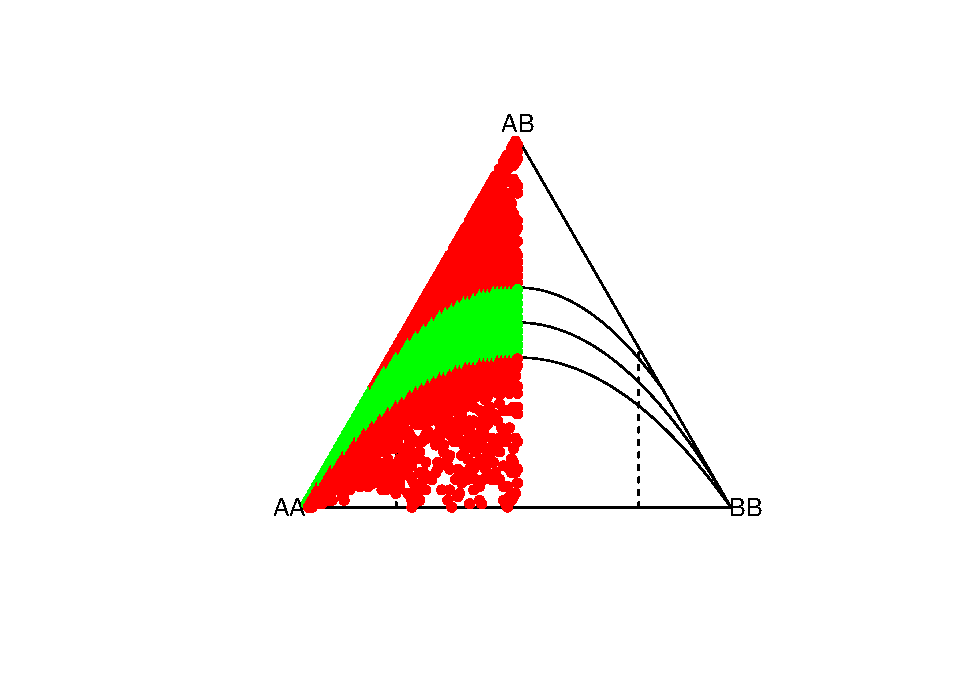
\includegraphics{P022020_HWE_files/figure-latex/12th-1.pdf}

\begin{enumerate}
\def\labelenumi{\arabic{enumi}.}
\setcounter{enumi}{12}
\tightlist
\item
  (1p) Can you explain why half of the ternary diagram is empty?
\end{enumerate}

Discussing the possibilities why the right part of the ternary diagram
is empty we came to the conclusion that A is probably always taken as
the more frequent allele and thus there is no way when BB could be a
more frequent case than AA.

\begin{enumerate}
\def\labelenumi{\arabic{enumi}.}
\setcounter{enumi}{13}
\tightlist
\item
  (2p) Make a histogram of the \(p\)-values obtained in the chi-square
  test. What distribution would you expect if HWE would hold for the
  data set? Make a Q-Q plot of the \(p\) values obtained in the
  chi-square test against the quantiles of the distribution that you
  consider relevant. What is your conclusion?.
\end{enumerate}

\begin{Shaded}
\begin{Highlighting}[]
\KeywordTok{hist}\NormalTok{(pvalues_chi, }\DataTypeTok{freq=}\OtherTok{FALSE}\NormalTok{)}
\KeywordTok{curve}\NormalTok{ (}\KeywordTok{dbeta}\NormalTok{(x, }\DataTypeTok{shape1 =} \DecValTok{80}\NormalTok{, }\DataTypeTok{shape2 =} \DecValTok{3}\NormalTok{), }\DataTypeTok{add=}\OtherTok{TRUE}\NormalTok{, }\DataTypeTok{col=}\StringTok{"red"}\NormalTok{)}
\end{Highlighting}
\end{Shaded}

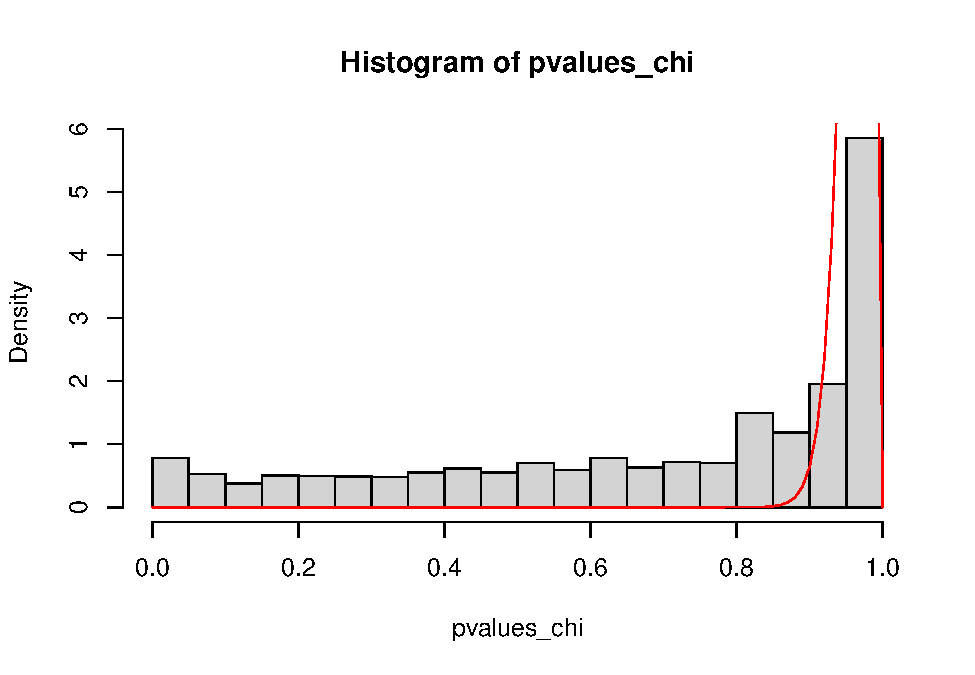
\includegraphics{P022020_HWE_files/figure-latex/14th-1.pdf}

\begin{Shaded}
\begin{Highlighting}[]
\NormalTok{x_qbeta <-}\StringTok{ }\KeywordTok{seq}\NormalTok{(}\DecValTok{0}\NormalTok{, }\DecValTok{1}\NormalTok{, }\DataTypeTok{length.out =} \KeywordTok{length}\NormalTok{(pvalues_chi))}
\NormalTok{y_qbeta <-}\StringTok{ }\KeywordTok{rbeta}\NormalTok{(x_qbeta, }\DataTypeTok{shape1 =} \DecValTok{80}\NormalTok{, }\DataTypeTok{shape2 =} \DecValTok{3}\NormalTok{)}

\KeywordTok{qqplot}\NormalTok{(pvalues_chi, y_qbeta, }\DataTypeTok{main=}\StringTok{"Q-Q plot"}\NormalTok{, }\DataTypeTok{xlab =} \StringTok{"P-values"}\NormalTok{, }\DataTypeTok{ylab =} \StringTok{"Beta distribution quantiles"}\NormalTok{)}
\end{Highlighting}
\end{Shaded}

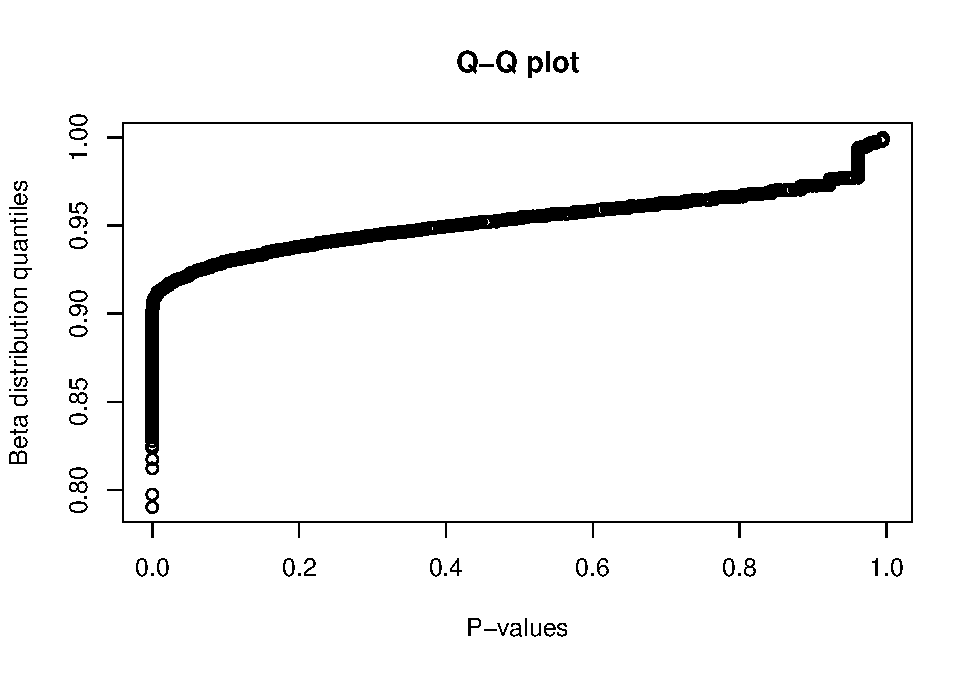
\includegraphics{P022020_HWE_files/figure-latex/14th-2.pdf}

If HWE would hold for the whole data set, we would expect that the left
part of the histogram (below 0.05) is 0, i.e.~that no row has p-value
below 0.05. Ideally we would expect the mass of the histogram to shift
as far right as possible.

This histogram is shaped like some very skewed distribution with heavy
left tail. We could not find some distribution with a heavy tail like
this, do the best fit for this is beta distribution with parameters
alpha = 80 and beta = 3. Q-Q plot is presented in the plot, we see that
in the middle there is linear behavior, but coming closer to each end of
the curve the points start to deviate significantly from the line.

\begin{enumerate}
\def\labelenumi{\arabic{enumi}.}
\setcounter{enumi}{14}
\tightlist
\item
  (1p) Imagine that for a particular marker the counts of the two
  homozygotes are accidentally interchanged. Would this affect the
  statistical tests for HWE? Try it on the computer if you want. Argue
  your answer.
\end{enumerate}

\begin{Shaded}
\begin{Highlighting}[]
\NormalTok{counts <-}\StringTok{ }\KeywordTok{c}\NormalTok{(}\DataTypeTok{AA=}\DecValTok{40}\NormalTok{, }\DataTypeTok{AB=}\DecValTok{10}\NormalTok{, }\DataTypeTok{BB=}\DecValTok{15}\NormalTok{)}
\KeywordTok{HWChisq}\NormalTok{(counts)}
\end{Highlighting}
\end{Shaded}

\begin{verbatim}
## Chi-square test with continuity correction for Hardy-Weinberg equilibrium (autosomal)
## Chi2 =  24.22897 DF =  1 p-value =  8.553578e-07 D =  -8.846154 f =  0.6388889
\end{verbatim}

\begin{Shaded}
\begin{Highlighting}[]
\NormalTok{interchanged_counts <-}\StringTok{ }\KeywordTok{c}\NormalTok{(}\DataTypeTok{AA=}\DecValTok{15}\NormalTok{, }\DataTypeTok{AB=}\DecValTok{10}\NormalTok{, }\DataTypeTok{BB=}\DecValTok{40}\NormalTok{)}
\KeywordTok{HWChisq}\NormalTok{(interchanged_counts)}
\end{Highlighting}
\end{Shaded}

\begin{verbatim}
## Chi-square test with continuity correction for Hardy-Weinberg equilibrium (autosomal)
## Chi2 =  24.22897 DF =  1 p-value =  8.553578e-07 D =  -8.846154 f =  0.6388889
\end{verbatim}

If counts of two homozygotes were accidentally interchanged, it wouldn't
affect the statistical test for HWE. Switching counts of two homozygotes
also switches the probabilities p and q, which does not change the test
value. It can be seen if we observe formula for Chi-squared test (on
slide 19 from the lesson's PDF). Heterozygote count does not change, so
the nominator stays equal. Denominator consists of factor
\emph{p-squared}, \emph{q-squared} and \emph{n} and stays equal if we
switch p and q values.

\begin{enumerate}
\def\labelenumi{\arabic{enumi}.}
\setcounter{enumi}{15}
\tightlist
\item
  (3p) Compute the inbreeding coefficient (\(\hat{f}\)) for each SNP,
  and make a histogram of \(\hat{f}\). You can use function \texttt{HWf}
  for this purpose. Give descriptive statistics (mean, standard
  deviation, etc) of \(\hat{f}\) calculated over the set of SNPs. What
  distribution do you expect \(\hat{f}\) to follow theoretically? Use a
  probability plot to confirm your idea.
\end{enumerate}

\begin{Shaded}
\begin{Highlighting}[]
\NormalTok{fs <-}\StringTok{ }\KeywordTok{HWf}\NormalTok{(}\KeywordTok{as.matrix}\NormalTok{(genotype_counts))}
\KeywordTok{hist}\NormalTok{(fs, }\DataTypeTok{freq=}\OtherTok{FALSE}\NormalTok{)}
\KeywordTok{curve}\NormalTok{ (}\KeywordTok{dnorm}\NormalTok{(x, }\FloatTok{-0.05}\NormalTok{, }\FloatTok{0.05}\NormalTok{), }\DataTypeTok{add=}\OtherTok{TRUE}\NormalTok{, }\DataTypeTok{col=}\StringTok{"red"}\NormalTok{)}
\end{Highlighting}
\end{Shaded}

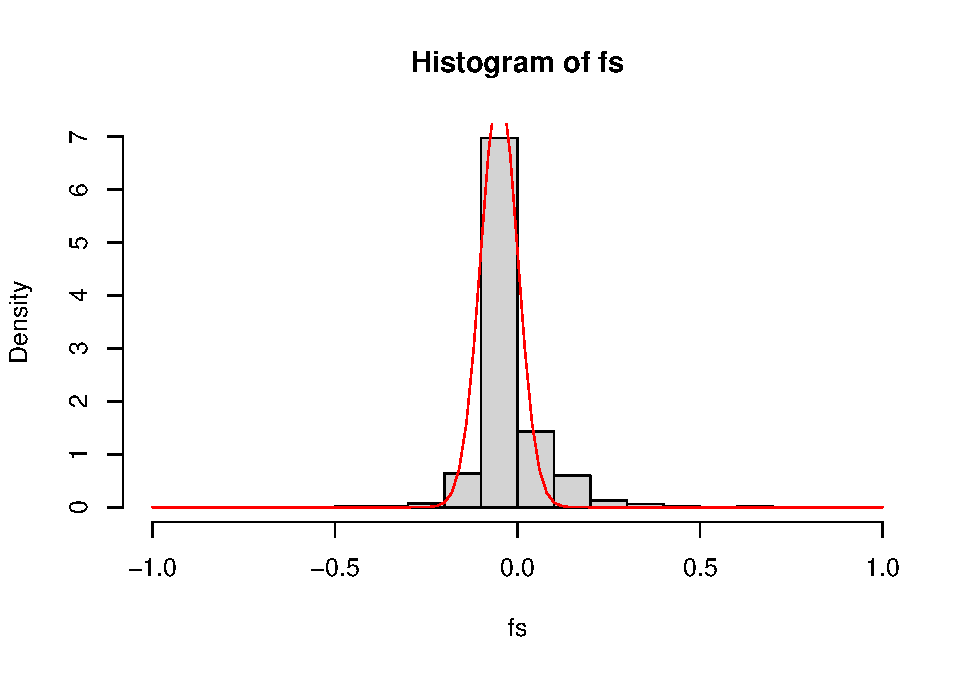
\includegraphics{P022020_HWE_files/figure-latex/16th-1.pdf}

\begin{Shaded}
\begin{Highlighting}[]
\KeywordTok{cat}\NormalTok{(}\KeywordTok{paste}\NormalTok{(}\StringTok{'Mean:'}\NormalTok{, }\KeywordTok{mean}\NormalTok{(fs), }\StringTok{'}\CharTok{\textbackslash{}n}\StringTok{Standard deviation:'}\NormalTok{, }\KeywordTok{sd}\NormalTok{(fs), }\StringTok{'}\CharTok{\textbackslash{}n}\StringTok{Median:'}\NormalTok{, }\KeywordTok{median}\NormalTok{(fs), }\StringTok{'}\CharTok{\textbackslash{}n}\StringTok{Min:'}\NormalTok{, }\KeywordTok{min}\NormalTok{(fs), }\StringTok{'}\CharTok{\textbackslash{}n}\StringTok{Max:'}\NormalTok{, }\KeywordTok{max}\NormalTok{(fs)))}
\end{Highlighting}
\end{Shaded}

\begin{verbatim}
## Mean: -0.00466823238593223 
## Standard deviation: 0.0950119986299748 
## Median: -0.00469483568075117 
## Min: -0.981481481481482 
## Max: 1
\end{verbatim}

Considering that the mean and the median are very similar values, and
looking at the histogram, it seems that inbreeding coefficients follow
normal distribution. Distribution with parameters N(-0.05, 0.05) seems
to make a good explanation of inbreeding coefficients distribution of
this data set.

\begin{enumerate}
\def\labelenumi{\arabic{enumi}.}
\setcounter{enumi}{16}
\tightlist
\item
  (2p) Make a plot of the observed chi-square statistics against the
  inbreeding coefficient (\(\hat{f}\)). What do you observe? Can you
  give an equation that relates the two statistics?
\end{enumerate}

\begin{Shaded}
\begin{Highlighting}[]
\KeywordTok{plot}\NormalTok{(pvalues_chi, fs)}
\end{Highlighting}
\end{Shaded}

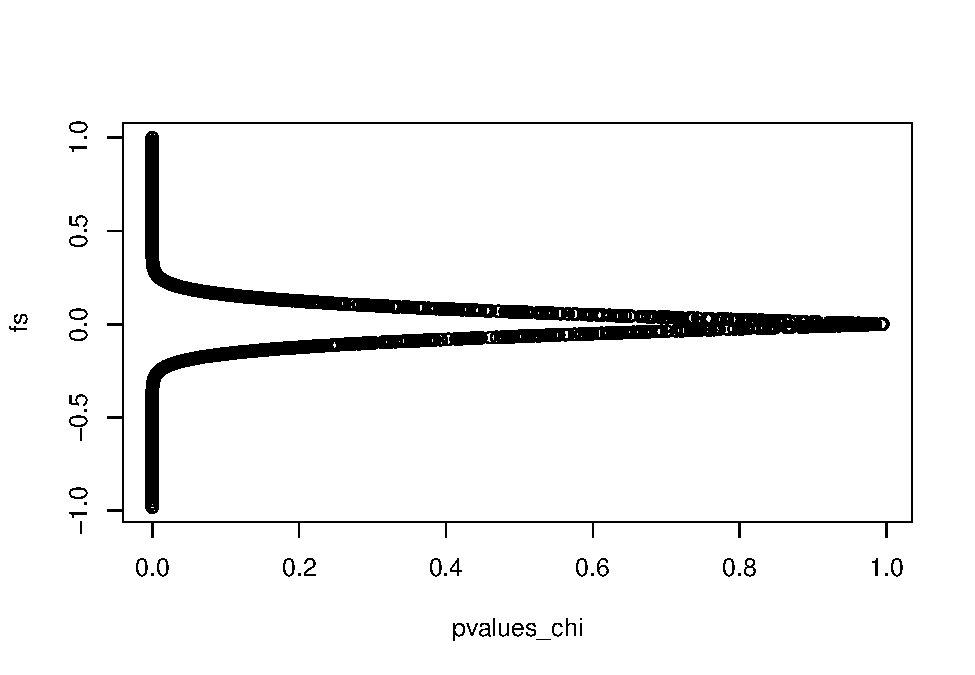
\includegraphics{P022020_HWE_files/figure-latex/17th-1.pdf} We can
observe that p-values are closer to zero as inbreeding coefficient is
further from zero, and vice versa. That makes sense, because low p-value
indicates that variant is not in equilibrium, and it happens when there
are no heterozygotes (f = 1) or much more heterozygotes than homozygotes
(f = -1).

\begin{enumerate}
\def\labelenumi{\arabic{enumi}.}
\setcounter{enumi}{17}
\tightlist
\item
  (2p) We reconsider the exact test for HWE, using different significant
  levels. Report the number and percentage of significant variants using
  an exac test for HWE with \(\alpha = 0.10, 0.05, 0.01\) and 0.001.
  State your conclusions.
\end{enumerate}

\begin{Shaded}
\begin{Highlighting}[]
\NormalTok{get_significant_percentage <-}\StringTok{ }\ControlFlowTok{function}\NormalTok{(pvalues, alpha) \{}
\NormalTok{  significant <-}\StringTok{ }\NormalTok{pvalues[pvalues }\OperatorTok{<=}\StringTok{ }\NormalTok{alpha]}
  \KeywordTok{length}\NormalTok{(significant) }\OperatorTok{/}\StringTok{ }\KeywordTok{length}\NormalTok{(pvalues)}
\NormalTok{\}}

\NormalTok{significant_percentages <-}\StringTok{ }\KeywordTok{c}\NormalTok{(}\KeywordTok{get_significant_percentage}\NormalTok{(pvalues_exact, }\FloatTok{0.10}\NormalTok{),}
                             \KeywordTok{get_significant_percentage}\NormalTok{(pvalues_exact, }\FloatTok{0.05}\NormalTok{),}
                             \KeywordTok{get_significant_percentage}\NormalTok{(pvalues_exact, }\FloatTok{0.01}\NormalTok{),}
                             \KeywordTok{get_significant_percentage}\NormalTok{(pvalues_exact, }\FloatTok{0.001}\NormalTok{))}
\KeywordTok{names}\NormalTok{(significant_percentages) <-}\StringTok{ }\KeywordTok{c}\NormalTok{(}\StringTok{'0.1'}\NormalTok{, }\StringTok{'0.05'}\NormalTok{, }\StringTok{'0.01'}\NormalTok{, }\StringTok{'0.001'}\NormalTok{)}
\NormalTok{significant_percentages}
\end{Highlighting}
\end{Shaded}

\begin{verbatim}
##         0.1        0.05        0.01       0.001 
## 0.048064322 0.027707893 0.011995753 0.007102748
\end{verbatim}

We can see that percentage of significant variants decreases as alpha is
approaching zero.

\end{document}
